\subsubsection{Output: The Instance Wise Dataflow Graph}
Sources of all read variables can be summarised in an instance wise dataflow graph. The dataflow graph produced by \verb|FADAtool| is generated in a \verb|.dot| format (or a \verb|.vcg| format according to the constant \verb|graph_format| in \verb|constants.h|), then automatically converted (if GraphViz installed) into an image. Currently, there is no other output format, we shall appreciate reporting any special format you want the dependence graph will be represented in. 

Here a part of the dataflow graph for the matrix multiply example (Figure~\ref{pgm:matmul}).
\begin{verbatim}
 $ fadatool -i MatMul.c -gc
\end{verbatim}

\begin{center}
 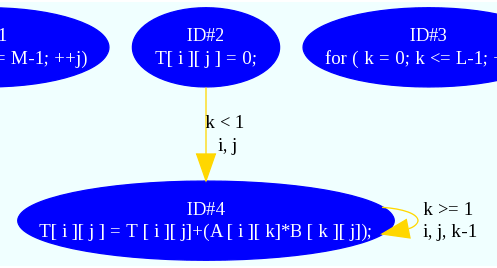
\includegraphics[scale=0.6]{MatMul_DFG.png}
 \end{center}
% \caption{An instance wise dependence graph for program in fig. \ref{pgm:matmul}}
% \label{fig:unfilled_dg}
% \end{figure}

On edges:
\begin{itemize}
 \item The first line gives the condition on validity of the dependence.
 \item The second line gives the function which define the source instance.
\end{itemize}

Here we assume that the read operations are executed during the current iteration vector. Dependent statement instances are identified by an affine function on the read iteration.\\
Let us observe the dependent operations with the operation \verb|ID#4| executed during the iteration \verb|(i, j, k)| (set as the current iteration). One of these dependent operations is \verb|ID#2| executed during the iteration \verb|(i, j)|, the other is another instance of \verb|ID#4| executed during \verb|(i, j, k-1)|.

